\documentclass[18pt]{beamer}
\usetheme{Madrid}

\usepackage{graphics}
\usepackage{listings}
\usepackage{url}
\usepackage{verbatim}
\usepackage{xcolor}

\lstset{language=C++,numbersep=1pt,identifierstyle=\color{blue!50!black},commentstyle=\color{yellow!50!black},xleftmargin=7pt,numberblanklines=false,numberstyle=\color{red!60!black},numbers=left,basicstyle=\tiny\ttfamily,keywordstyle=\color{green!60!black}\bfseries,stringstyle=\color{red!80!black}}

\newcommand{\lstlistingwithnumber}[3]{
\begin{center}
\lstinputlisting[linerange={#1-#2},firstnumber=#1]{#3}
\end{center}
}

\newcommand{\centeredlargetext}[3]{
{
\setbeamertemplate{background}{}
\setbeamertemplate{navigation symbols}{}
\setbeamercolor{background canvas}{bg={#1}}
\color{#2}
\begin{frame}[plain]
\fontsize{36pt}{36pt}\selectfont
\center
\begin{center}
{#3}
\end{center}
\end{frame}
}}

\newcommand{\centeredhugetext}[3]{
{
\setbeamertemplate{navigation symbols}{}
\setbeamercolor{background canvas}{bg={#1}}
\fontsize{72pt}{72pt}\selectfont
\color{#2}
\begin{frame}[plain]
\center
\begin{center}
{#3}
\end{center}
\end{frame}
}}


\begin{document}

\title[ANTsMM]{Multi-modality processing with \newline Advanced Normalization
  Tools (ANTs)}
\subtitle[ANTsMM]{Modern data fusion strategies}
\institute[PICSL]{Brian Avants, PICSL and the ANTs Development Team}
\date

\begin{frame}
\titlepage
\end{frame}


{
\setbeamertemplate{navigation symbols}{}
\begin{frame}[plain]
\center
\begin{center}
This presentation is copyrighted by\\
The \textbf{ANTs software consortium}\\
\bigskip
distributed under the\\
\textbf{Creative Commons by Attribution License 3.0}\\
\url{http://creativecommons.org/licenses/by/3.0}\\
\end{center}
\end{frame}
}


% \begin{frame}
%  \tableofcontents[hideallsubsections]
% \end{frame}

% \setbeamertemplate{background}{
\includegraphics[width=\paperwidth]{../figures/ITKv4_transparent}}
\setbeamertemplate{background}{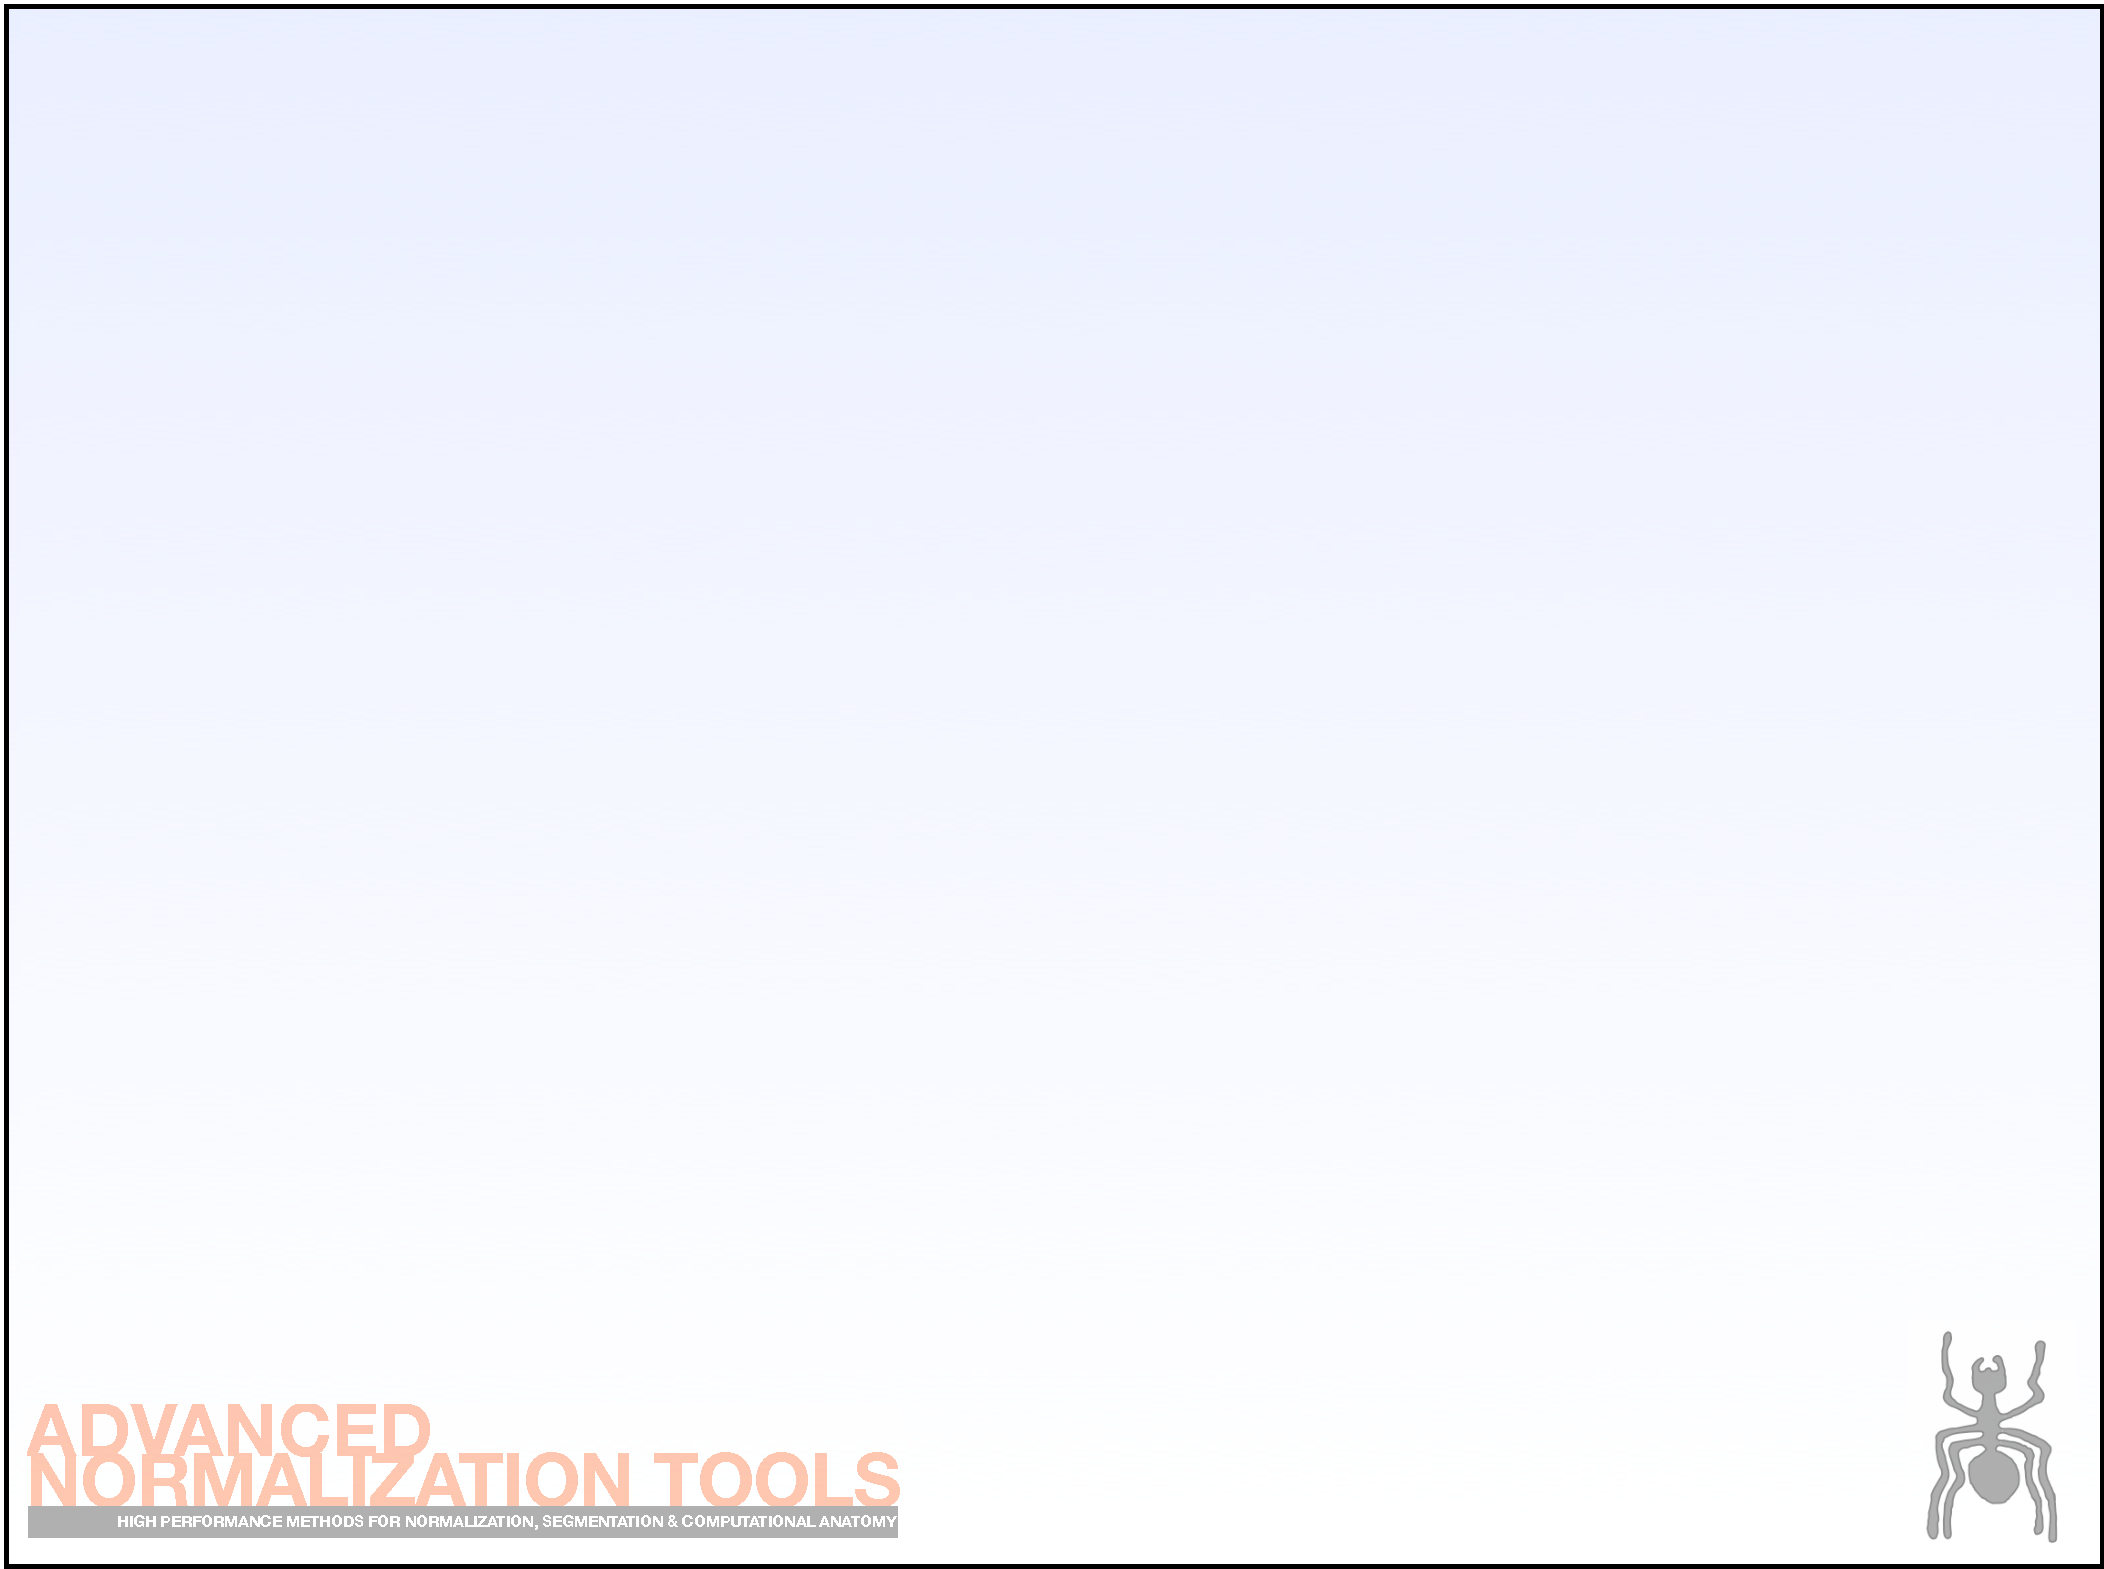
\includegraphics[width=\paperwidth]{../figures/ants_background.pdf}}


\begin{frame}
\frametitle{People}
nick, gang, niels, shrinidhi ...
\end{frame}

\begin{frame}
\frametitle{History}
ants history + relationship to ITK ( bidirectional )
\end{frame}

\begin{frame}
\frametitle{Overview}
ants overview of tools :  multivariate registration, segmentation, bias correction, template building and image-math 
\end{frame}

\begin{frame}
\frametitle{Scripting}
ants is for scripting 
\end{frame}

\begin{frame}
\frametitle{Basic Toolset}
ants-essential tools:  a mapping, a segmentation, a template and then label-guided and multivariate versions of these.  
\end{frame}

\begin{frame}
\frametitle{Basic applications}
ants-based studies:  ROI study of thickness, template-study of thickness/gmprob,  template-study of FA, multi-modality study, bold fmri study, asymmetry study.   dimensionality reduction.  
\end{frame}


\begin{frame}
\frametitle{Segmenting an image}
standard ants call 
\end{frame}

\begin{frame}
\frametitle{Segmenting an image with two modalities}
r16 plus an edge map ... 
\end{frame}

\begin{frame}
\frametitle{Meaning of parameters}
what happens when i vary each parameter?
\end{frame}

\begin{frame}
\frametitle{Cortical thickness}
r16 thickness 
\end{frame}

\begin{frame}
\frametitle{Meaning of parameters}
what happens when i vary each parameter?
\end{frame}

\begin{frame}
\frametitle{Mapping two images}
standard ants call 
\end{frame}

\begin{frame}
\frametitle{Meaning of parameters}
what happens when i vary each parameter?
\end{frame}

\begin{frame}
\frametitle{Coordinates of computation time}
2D MSQ to 3D CC
\end{frame}

\begin{frame}
\frametitle{Landmark-based registration}
Schoenemann examples affine + bspline 
\end{frame}

\begin{frame}
\frametitle{Multiple metrics driving registration}
face example and why we use LMs @ the same time as data 
\end{frame}

\begin{frame}
\frametitle{Template construction}
group studies 
\end{frame}

\begin{frame}
\frametitle{Templates for asymmetry analysis}
chimpanzee cortical thickness 
\end{frame}

\begin{frame}
\frametitle{Templates for all modalities}
what is common?  brain
\end{frame}

\begin{frame}
\frametitle{Longitudinal analysis with ANTs}
script based 
\end{frame}

\begin{frame}
\frametitle{Time series / rsfMRI analysis with ANTs}
script based 
\end{frame}

\begin{frame}
\frametitle{Statistical analysis with ANTs}
script based 
\end{frame}

\begin{frame}
\frametitle{How does structure and functional connectivity elaborate during development?}
open data
\end{frame}


\begin{frame}
\frametitle{Reproducibility}
\Huge
\begin{itemize}
\item a
\pause
\item study
\pause
\item slide
\pause
\item Reproducible Research!
\end{itemize}
\end{frame}


\end{document}



ants multivariate tutorial

implement with beamer : github, scripts, figures, etc

pauly:  pointset matching with b-splines 

hongzhi:  I will be interested to know how to incorporate additional information, such as landmarks, other than images to help registration, how to build atlases and do groupwise registration with ANTS

JJ data as guide + ADNI for longitudinal processing 


graph analysis

I'm most interested in relating structural images to continuous behavioral measures - for example, age, the amount of improvement on a behavioral task, or the level of some CSF analyte (I'm assuming the analysis would be essentially identical for any continuous measure...).


--- asymmetry is important 

